\section{Evaluation} \label{evaluation}
\begin{table}[t]
	\begin{tabular}{l*{4}{c}}
		\toprule
		\multirow{2}{*}{\bfseries Benchmarks} & \multicolumn{2}{c}{\bfseries \begin{tabular}{@{}l@{}} Normalized \\ with Baseline \end{tabular}} & \multicolumn{2}{c}{\bfseries \begin{tabular}{@{}l@{}} Normalized \\ with SafeStack \end{tabular}} \\%& \multirow{2}{*}{\bfseries \begin{tabular}{@{}l@{}} Number of tracking \\ functions inserted \end{tabular}} \\ % Great ;) hack to insert new line a cell
				
		\hhline{~----} & \begin{tabular}{@{}l@{}} Heap \\ Pointers \end{tabular} & \begin{tabular}{@{}l@{}} All \\ Pointers \end{tabular} & \begin{tabular}{@{}l@{}} Heap \\ Pointers \end{tabular} & \begin{tabular}{@{}l@{}} All \\ Pointers \end{tabular} \\ 
		\toprule
    		
    		\csvreader[head to column names]{Tables/spec_num.csv}{} % use head of csv as column names	
    		{\\\benchmark & \heapptrbaseline & \allptrbaseline & \heapptrsafestack & \allptrsafestack }%& \numinst} % specify coloumns here
    		\\
    		\bottomrule
	\end{tabular}
	
	\caption{SPEC2006 run-time overhead normalized with baseline and baseline-safestack. \projectname{} has $53\%$ run-time overhead compared to baseline numbers when only heap pointers are tracked, whereas $43\%$ compared to baseline-safestack. It has only $4\%$ more degradation when all pointers (Stack, Heap and Global) are tracked compared to when only heap pointers are tracked.}
	\label{table:spec2006}
	%\vspace{-1em}
\end{table}

\begin{figure}[t]
\center
  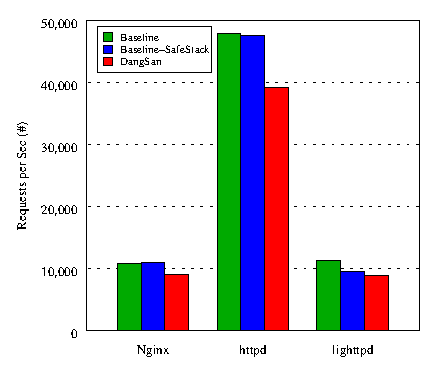
\includegraphics[width=3in]{plots/server_perf.eps}
  \caption{Web servers throughput degradation when compiled with \projectname{}. On an average throughput degradation is $12.8\%$ (compared to baseline-safestack). Negligible degradation in service latency.}
 \label{fig:server_perf}
  \vspace{-1em}
\end{figure} 

We evaluated \projectname{} in terms of performance overhead and effectiveness. We used CPU-intensive SPEC2006 performance benchmarks. For baseline configuration, we compiled benchmarks with clang/LLVM $3.8.0$. Moreover, we took numbers with one more baseline configuration (\emph{baseline-safestack}) with SafeStack option enabled. \metalloc{} handles stack objects similar to SafeStack. However, \projectname{} do not track stack objects. Therefore, we compare \projectname{} with baseline-safestack to remove run-time overhead introduced by stack objects handling. Both baseline configurations use unmodified \texttt{tcmalloc 4.2.6}~\cite{ghemawat2009tcmalloc} as a custom memory allocator. For \projectname{}, we compiled applications with our extra LLVM transformation pass to instrument the code. We linked \projectname{} run-time library statically with the application. We used custom inliner LLVM pass to inline most of the our run-time tracking functions. For all configurations, compiler optimization is set to \texttt{-O3}. We ran benchmarks on $64$-bit CentOS Linux with Intel Xeon CPU E5-2640 v3. We kept value of $\emph{N}\ =\ 3$, baselog size$\ =\ 8$ (number of pointers) with exponential log resize strategy.

\subsection{Performance Analysis} 
%\csvautotabular{Tables/spec_num.csv}

%%%%% Make comment for adding new line to the cell. Remove the hack

Table~\ref{table:spec2006} depicts run-time overhead of SPEC2006 benchmarks. Benchmark run-times are normalized with baseline and baseline-safestack. Stack pointers are short lived. That is, attacker has a very short time to exploit vulnerability. Use-after-Free exploits using stack dangling pointers are very rare. Performance overhead of tracking stack pointers is very high compared to its benefit. Therefore, we performed experiments for tracking all pointers (Stack, Heap and Global) and only heap pointers. Our static instrumentation has conservative approach. We end up instrumenting every pointer store instruction. We skip registration for invalid pointers and objects during run-time. This reduces large number of false negatives.  \projectname{} has average performance degradation (\textit{geomean}) of $53\%$ when only heap pointers are tracked. Moreover, it has only $4\%$ more (compared to only heap pointers tracking) overhead when all pointers are tracked. SafeStack has low performance degradation of $0.1\%$ ~\cite{kuznetsov2014code}. Compared to baseline-safestack, \projectname{} has average performance degradation of $44\%$ when only heap pointers are tracked. Similar to baseline, it has only $4\%$ more (compared to only heap pointers tracking) overhead when all pointers are tracked. \texttt{omnetpp} and \texttt{perlbench} have high performance degradation of $6x$ and $4x$ times, respectively. State-of-the-art Use-after-Free detection schemes have not included either \texttt{omnetpp} or \texttt{perlbench} overhead. Therefore, we cannot directly compare our average performance overhead with other recent schemes. When \texttt{omnetpp} is excluded, average performance overhead is $42\%$ (normalized with baseline) and $39\%$ (normalized with baseline-safestack) when all pointers are tracked. \\
% Include number of instruction instrumented %

% Server numbers and graph %/
Moreover, we evaluated \projectname{} on widely used web servers like \texttt{nginx}, \texttt{httpd} and \texttt{lighttpd}. We measured service latency (runtime) and throughput (Number of requests per sec) degradation. To measure service latency, we downloaded $2$GB file from server to client on localhost. We took average of $11$ runs. \projectname{} has shown negligible service latency degradation. To measure throughput, we used \texttt{ApacheBench}. We triggered $25000$ requests for static \texttt{index} page using $10$ concurrent requests. Figure~\ref{fig:server_perf} shows throughput degradation compared to baseline and baseline-safestack. \texttt{lighttpd} has low throughput degradation of $6.5\%$, whereas \texttt{nginx} and \texttt{httpd} has moderate degradation of $18.2\%$ and $17.7\%$, respectively. On an average (geomean), Web Servers have $12.8\%$ throughput degradation compared to baseline-safestack.     \\

% Run-time stats to explain more numbers
\begin{table*}[t]
\center
\begin{tabular}{l|*{6}{r}}
	\toprule
	\tablecell{Benchmarks} & \tablecell{Number of tracking \\ calls inserted} & \tablecell{Pointer \\ Registrations} & \tablecell{Duplicate \\ Pointers (\%)} & \tablecell{Objects \\ Allocated} & \tablecell{Objects \\ Free (\%)} & \tablecell{Log \\Overflows} \\
	\toprule
	\csvreader[head to column names]{Tables/spec_stats1.csv}{}
	{\\\benchmarks & \numinst & \ptrreg & \dupptr & \objalloc & \objfree & \logflow} \\% specify coloumns here
	\bottomrule
\end{tabular}
\caption{Run-time statistics for the SPEC2006 benchmarks}
\label{table:spec_stats}
\end{table*}

Furthermore, we collected run-time statistics to understand performance degradation. For this, we instrumented \projectname{} run-time library functions. Table~\ref{table:spec_stats}\ depict runtime statistics for SPEC2006 benchmarks compiled with \projectname{}. Column $2$ (Number of tracking calls inserted) represents a number of store instructions instrumented during static instrumentation phase. We have conservative static instrumentation pass. Therefore, we may end up instrumenting more than required. \texttt{gcc} and \texttt{xalancbmk} benchmark have almost $28K$ instrumented store instructions. Number of instrumented store instructions represent the number of pointer assignments found statically in the application. Column $3$ (Pointer Registrations) denotes a number of times run-time pointer tracking function is called. \texttt{gcc} and \texttt{xalancbmk} have more number of instrumented stores than \texttt{perlbench} and \texttt{omnetpp}. However, the number of run-time pointer tracking function calls are less. This is because same instrumented tracking function is called many times. It can happen when we instrument frequently executing application functions or loops. This information can be used to perform \projectname{} optimizations. Column $6$ represents number of allocated objects that are freed. Column $7$ shows the number of times log overflow occurred. Column $4$ shows percentage of  pointer registrations that are for \textit{Duplicate} pointers. For \texttt{lbm} benchmark, almost all pointer registrations are duplicates. For \texttt{sjeng} benchmark, pointer registrations are high with zero duplicates. It has only $5$ allocated objects and no log overflow. It can happen when pointer registration is called for a large number of invalid objects (Stack or Global) or pointers. \texttt{perlbench} and \texttt{omnetpp} have large number of object allocations and deallocations. Therefore, performance overhead for these benchmarks could be because of object allocations/deallocations. We initialize object metadata in allocation function and invalidate pointers in deallocation function. However, \texttt{dealII} and \texttt{xalancbmk} benchmark have more number of object allocations and deallocations than \texttt{perlbench}. Thus, performance overhead in \texttt{perlbench} seems to come from a large number pointer tracking function calls. As discussed earlier, these calls are from frequently executed application functions or loops. Therefore, advanced static instrumentation is required to avoid instrumentation for invalid store instructions. \\
%TODO Add for omnetpp

\textbf{Pointer Patterns.} 
We do not remove pointer registration from old objects metadata. Therefore, object log has large number of \emph{Duplicate} and \emph{Stale} pointers. We studied pointer pattern distribution (the number of \textit{Duplicate}, \textit{Unique} and \textit{Stale} pointers) in the log to fine-tune DangSan parameters.

\begin{figure*}[t]
\center
  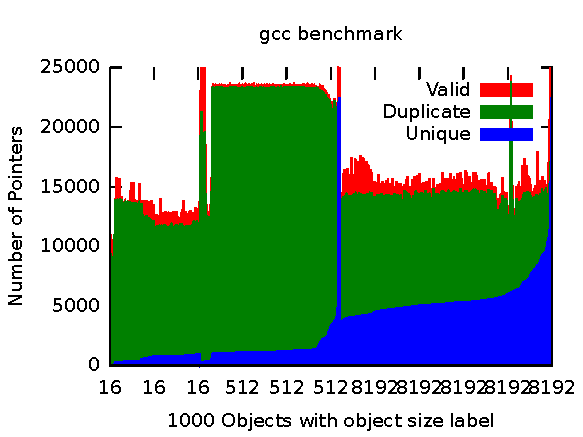
\includegraphics[width=2.8in,height=2.4in,keepaspectratio]{plots/gcc_pointerpattern.pdf}
  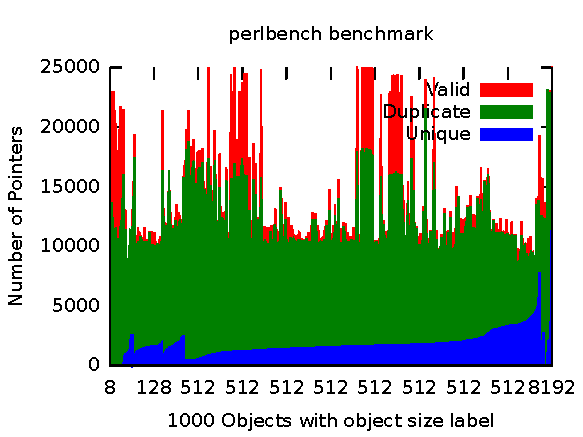
\includegraphics[width=2.8in,height=2.4in,keepaspectratio]{plots/perlbench_pointerpattern.pdf}
  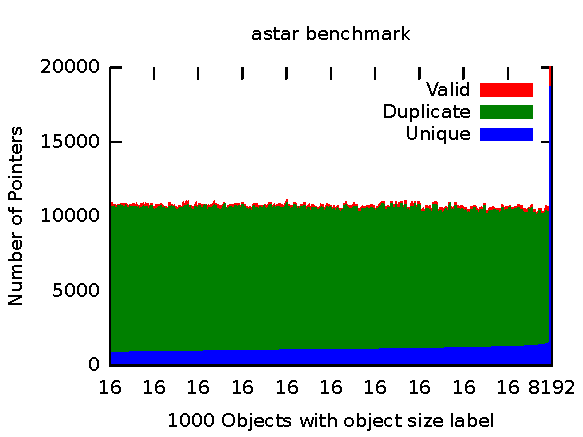
\includegraphics[width=2.8in,height=2.4in,keepaspectratio]{plots/astar_pointerpattern.pdf}
  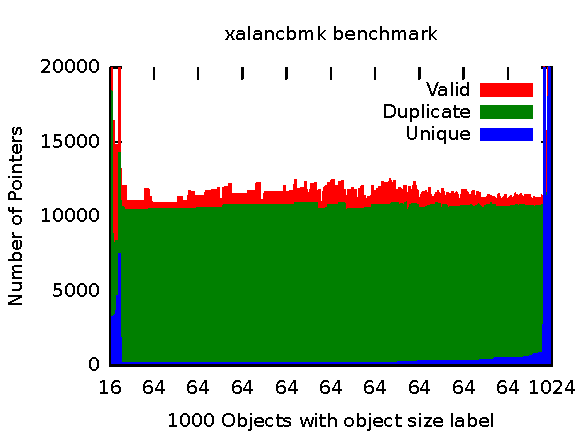
\includegraphics[width=2.8in,height=2.4in,keepaspectratio]{plots/xalancbmk_pointerpattern.pdf}
  
  \caption{Pointer registration pattern for the benchmarks that incur huge overhead. First $1000$ baselog overflow numbers are collected. N-Lookbehind value is $4$. Size of the baselog is kept very high to clearly visualize pattern difference.}
  \label{fig:pointerpattern}
  \vspace{-1em}
\end{figure*} 

Figure~\ref{fig:pointerpattern} shows pointer pattern distribution when a baselog overflow. We collected pointer pattern for first $1000$ objects that have overflown. The graph is plotted with increasing object size. Moreover, we collected statistics for benchmarks that incur huge overhead. Therefore, we chose two C benchmarks (\texttt{gcc} and \texttt{perlbench}) and two C++ benchmarks (\texttt{astar} and \texttt{xalancbmk}). We set baselog size to a very high value, $8K$ (number of pointers). Setting baselog size to a high value makes pattern clearly visible. We used \emph{N}-lookbehind value as $4$. In Figure~\ref{fig:pointerpattern}, red, green and blue area represents \textit{Valid}, \textit{Duplicate} and \textit{Unique} pointers, respectively. All four benchmarks have large number of \textit{Duplicate} pointers for any object size. Even after setting \emph{N}-Lookbehind value to $4$, \textit{Duplicate} pointers count is very high. Increasing value of \emph{N} may decrease \textit{Duplicate} pointers count but it has to trade-off with performance degradation. Furthermore, \emph{Unique} pointers count increases with object size for all the four benchmarks. Therefore, default baselog size should be proportional to the object size. However, it may introduce huge memory overhead. Next, the sum of \textit{Duplicate} and \textit{Unique} pointers represent the total number of pointers in the log. We store at max three pointers per log slot. Therefore, the total number of pointers per log can be at max $8K\ (log size) \times 3 = 24K$. For all the four benchmarks, on an average the total pointers count is above $11000$. In \texttt{gcc}, total pointers count reaches $23K$ for the object size $512$. That is, three times improvement in the memory utilization. Also, \textit{Valid} pointers count is very low for all the four benchmarks. Note, \textit{Valid} pointers count is inflated because pointers that are \textit{Duplicate} and \textit{Valid} are counted more than once. \textit{Valid} pointers count is very low even after counting \textit{Duplicate} and \textit{Valid} pointers more than once. Therefore, we need garbage collection of \textit{Stale} pointers to free the log space. \\

Furthermore, some pointers point to the same object but at different offset. These duplicate pointers may escape \emph{N}-Lookbehind strategy. We introduced one more strategy to remove these duplicate pointers. We compare old pointer value to the new object address range. When pointer points to the same object, we skip pointer registration. This \textit{Duplicate} pointers removal technique not only helps to remove \textit{Duplicate} pointers within a thread but also across threads. This technique removed $20\%\ to\ 25\%$ \emph{Duplicate} pointers for SPEC2006 benchmarks. For this technique, we need old pointer value in run-time tracking function. We slightly changed our static instrumentation pass. We insert run-time tracking function before store instruction instead of after store instruction. In run-time tracking function, we read old pointer value and check whether it still points to the same object. For fast check, we store object bound information in the object metadata. We store lowermost $32$-bits of object root address and object size together in the $64$-bit object metadata field. Therefore, \metalloc{} stores and retrieves $16$ bytes metadata, $8$ bytes for a pointer to a per-Thread log list and $8$ bytes for object information. \\

\subsection{Correctness}
We evaluated \projectname{} correctness on publicly available exploits. We chose following Use-after-Free (Double free) vulnerabilities. \\

\textbf{CVE-2010-­2939}~\cite{OpenSSLCVE}: This is a double free vulnerability in OpenSSL client version OpenSSL1.0.0a and function \texttt{ssl3\_get\_key\_exchange}. It is a highly critical vulnerability that results into denial of service or possible arbitrary code execution. We used exploit with the baseline configuration. It resulted into memory corruption error messages. Furthermore, we compiled OpenSSL1.0.0a with \projectname{}. We tried to exploit the compiled OpenSSL client. However, our system prevented double free. It aborted OpenSSL client due to invalid memory access.
\begin{verbatim}
src/tcmalloc.cc:290] Attempt to free invalid 
pointer 0x80000000022ba510 
./runclient: line 9: 20200 Aborted 
\end{verbatim} 
Above message indicates that our system had invalidated pointer by setting uppermost bit to $1$ when the object was freed first time.
 
\subsection{Memory Overhead}  
% Run-time stats to explain more numbers
\begin{table}[t]
\center
\begin{tabular}{l|*{3}{r}}
	\toprule
	\tablecell{Benchmarks} & \tablecell{Baseline \\RSS} & \tablecell{DangSan \\RSS} & \tablecell{Memory \\Overhead(MB)} \\
	\toprule
	\csvreader[head to column names]{Tables/spec_memory.csv}{}
	{\\\benchmarks & \baselinerss & \dangrss & \extramemory} \\% specify coloumns here
	\bottomrule
\end{tabular}
\caption{Memory overhead for the SPEC2006 benchmarks (MB)}
\label{table:spec_memory}
\end{table}

Table~\ref{table:spec_memory}\ shows memory overhead on SPEC2006 benchmarks introduced by \projectname{}. \texttt{perlbench}, \texttt{omnetpp}, \texttt{xalancbmk} and \texttt{astar} benchmarks have huge memory overhead in gigabytes. Memory overhead also comes from the metadata management scheme, \metalloc{}. \metalloc{} stores and retrieves $16$ bytes metadata for each object. It maintains metadata for all objects (including Stack and Global). We do not track Stack and Global objects. Thus, maintaining $16$ bytes metadata for Stack and Global object can inflate memory overhead numbers. Some defences may not require stack or global metadata management. One of the improvement required in \metalloc{} is to have selective metadata management. We believe that ~\metalloc{} will be used for other defences along with \projectname{}. Another reason for the memory overhead is, we increase one byte for every object allocation to solve \textbf{off-by-one} byte application compatibility issue. However, \texttt{tcmalloc} allocates object with powers of $2$ size. This tremendously increases memory overhead. One improvement to reduce memory overhead is to select additive increase log resize strategy. Table~\ref{table:spec_memory} also represents that increase in memory requirement increases performance overhead. This is directly proportional to the number of pointer propagations and object allocations. 